\begin{figure*}[hbtp]
  \centering
  \subfigure{
    \label{fig:cases-naive}
    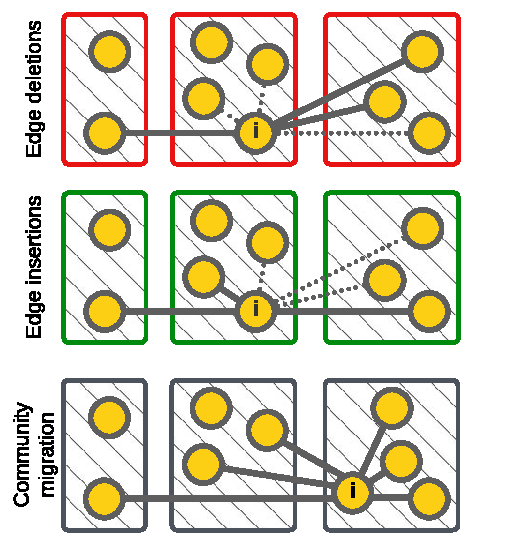
\includegraphics[width=0.3\linewidth]{out/about-cases-naive.pdf}
  }
  \subfigure{
    \label{fig:cases-delta-}
    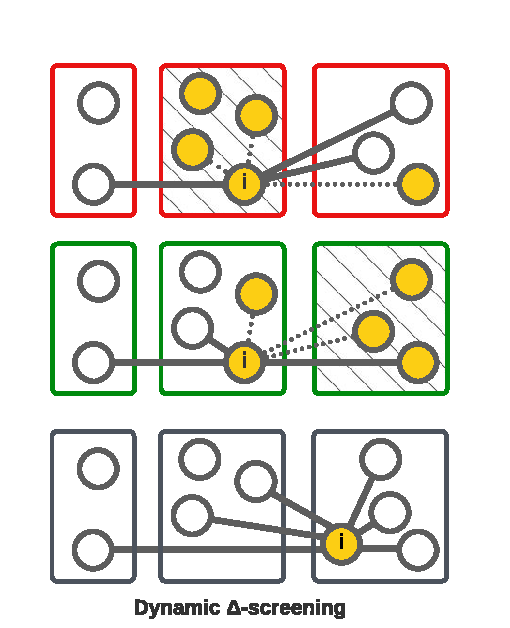
\includegraphics[width=0.3\linewidth]{out/about-cases-delta.pdf}
  }
  \subfigure{
    \label{fig:cases-frontier}
    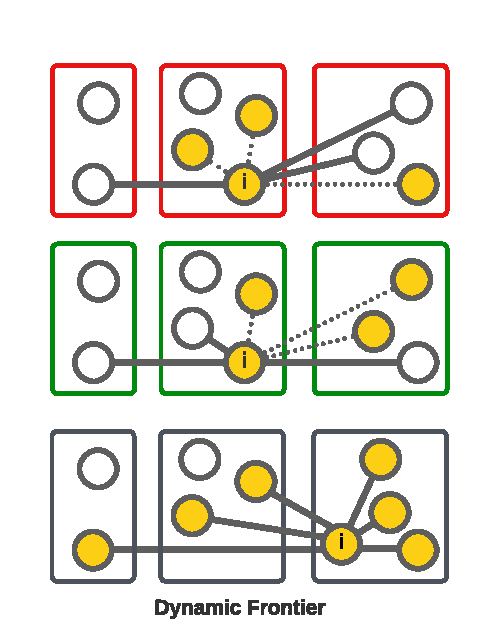
\includegraphics[width=0.3\linewidth]{out/about-cases-frontier.pdf}
  } \\[-2ex]
  \caption{Comparison of dynamic community detection approaches: \textit{Naive-dynamic} (\Nai{}), \textit{Dynamic $\Delta$-screening} (\Del{}), and \textit{Dynamic Frontier} (\Fro{}). Vertices marked as affected (initially) with each approach are highlighted in yellow, and when entire communities are marked as affected, they are hatched.}
   % Pre-existing edges are indicated with single-solid lines. Edge deletions in a batch update are shown by double-dashed lines (top), edge insertions are shown with double-solid lines (middle), and community migration of a vertex is shown with an arrow (bottom). Here $i$ represents a source vertex of edge deletions/insertions in the batch update, or a vertex that changes its community membership during the running of the community detection algorithm. Vertices marked as affected (initially) with each approach are highlighted in yellow, and when entire communities are marked as affected, they are hatched.
  \label{fig:dynamic-approaches}
\end{figure*}
